%%%%%%%%%%%%%%%%%%%%%%%%%%%%%%%%%%%%%%%%%
% Beamer Presentation
% LaTeX Template
% Version 1.0 (10/11/12)
%
% This template has been downloaded from:
% http://www.LaTeXTemplates.com
%
% License:
% CC BY-NC-SA 3.0 (http://creativecommons.org/licenses/by-nc-sa/3.0/)
%
%%%%%%%%%%%%%%%%%%%%%%%%%%%%%%%%%%%%%%%%%

%----------------------------------------------------------------------------------------
%	PACKAGES AND THEMES
%----------------------------------------------------------------------------------------

\documentclass{beamer}

\mode<presentation> {

% The Beamer class comes with a number of default slide themes
% which change the colors and layouts of slides. Below this is a list
% of all the themes, uncomment each in turn to see what they look like.

%\usetheme{default}
%\usetheme{AnnArbor}
%\usetheme{Antibes}
%\usetheme{Bergen}
%\usetheme{Berkeley}
%\usetheme{Berlin}
%\usetheme{Boadilla}
%\usetheme{CambridgeUS}
%\usetheme{Copenhagen}
%\usetheme{Darmstadt}
%\usetheme{Dresden}
%\usetheme{Frankfurt}
%\usetheme{Goettingen}
%\usetheme{Hannover}
%\usetheme{Ilmenau}
%\usetheme{JuanLesPins}
%\usetheme{Luebeck}
\usetheme{Madrid}
%\usetheme{Malmoe}
%\usetheme{Marburg}
%\usetheme{Montpellier}
%\usetheme{PaloAlto}
%\usetheme{Pittsburgh}
%\usetheme{Rochester}
%\usetheme{Singapore}
%\usetheme{Szeged}
%\usetheme{Warsaw}

% As well as themes, the Beamer class has a number of color themes
% for any slide theme. Uncomment each of these in turn to see how it
% changes the colors of your current slide theme.

%\usecolortheme{albatross}
%\usecolortheme{beaver}
%\usecolortheme{beetle}
%\usecolortheme{crane}
%\usecolortheme{dolphin}
%\usecolortheme{dove}
%\usecolortheme{fly}
%\usecolortheme{lily}
%\usecolortheme{orchid}
%\usecolortheme{rose}
%\usecolortheme{seagull}
%\usecolortheme{seahorse}
%\usecolortheme{whale}
%\usecolortheme{wolverine}

\usepackage{array}
\usepackage{amsmath}
%\defmathfamilydefault{rmdefault}
\usefonttheme[onlymath]{serif}
\usepackage{amssymb}
\DeclareMathOperator*{\argmax}{argmax}
\DeclareMathOperator*{\argmin}{argmin}

\usepackage{bm}

%\setbeamertemplate{footline} % To remove the footer line in all slides uncomment this line
%\setbeamertemplate{footline}[page number] % To replace the footer line in all slides with a simple slide count uncomment this line

%\setbeamertemplate{navigation symbols}{} % To remove the navigation symbols from the bottom of all slides uncomment this line
}

\usepackage{graphicx} % Allows including images
\usepackage{booktabs} % Allows the use of \toprule, \midrule and \bottomrule in tables
\usepackage{caption}

%----------------------------------------------------------------------------------------
%	TITLE PAGE
%----------------------------------------------------------------------------------------

\title[ ]{Linear Models for Regression} % The short title appears at the bottom of every slide, the full title is only on the title page

\author{Yan Yan} % Your name
\institute[SIAT] % Your institution as it will appear on the bottom of every slide, may be shorthand to save space
{
Shenzhen Institute of Advanced Technology\\
Chinese Academy of Sciences \\ % Your institution for the title page
\medskip
{yan.yan@siat.ac.cn} % Your email address
}
\date{September 30, 2016} % Date, can be changed to a custom date

\begin{document}

\begin{frame}
\titlepage % Print the title page as the first slide
\end{frame}

\begin{frame}
\frametitle{Overview} % Table of contents slide, comment this block out to remove it
\tableofcontents % Throughout your presentation, if you choose to use \section{} and \subsection{} commands, these will automatically be printed on this slide as an overview of your presentation
\end{frame}

%----------------------------------------------------------------------------------------
%	PRESENTATION SLIDES
%----------------------------------------------------------------------------------------

%------------------------------------------------
\section{Linear Basis Function Models} % Sections can be created in order to organize your presentation into discrete blocks, all sections and subsections are automatically printed in the table of contents as an overview of the talk
%------------------------------------------------

%\subsection{Subsection Example} % A subsection can be created just before a set of slides with a common theme to further break down your presentation into chunks

\begin{frame}
\frametitle{Linear Basis Function Models}


 The simplest linear model for regression (often simply known as \textit{linear regression}):
\begin{equation}
y(\bm{x},\bm{w})=\omega_0+\omega_1x_1+\cdots+\omega_Dx_D = \sum_{j=0}^{M-1}\omega_j\phi_j(\bm{x})=\bm{\omega}^T\phi(x)
\end{equation}
where $\bm{\omega}=(\omega_0,...,\omega_{M-1})^T$ and $\bm{\phi}=(\phi_0,\cdots,\phi_{M-1})^T$. This kinds of models are called linear models.\\~\\

 When $\phi$ has different types, which means different kinds of \textit{basis function}, we have other kinds of modes, like:
\begin{equation}
\phi_j(x) = exp\{-\frac{(x-\mu_j)^2}{2s^2}\}
\end{equation}

or
\begin{equation}
\phi_j(x) = \sigma(\frac{x-\mu_j}{s}) \quad and \quad \sigma(a) = \frac{1}{1+exp(-a)}
\end{equation} 

\end{frame}

\begin{frame}
\frametitle{Examples of basis function}
\begin{figure}
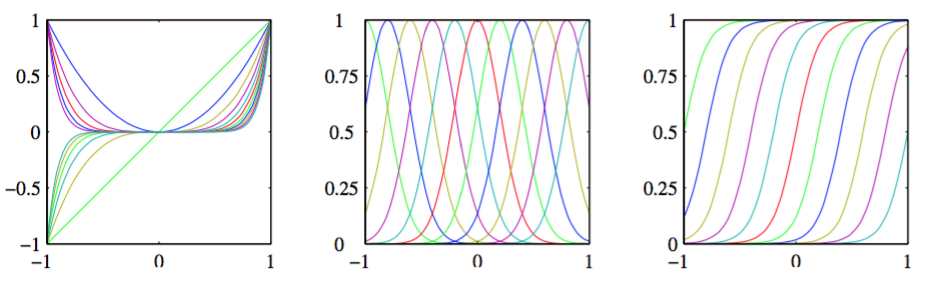
\includegraphics[width=12cm]{Figure1}
\caption{Examples of basis functions.}
%\label{Figure1}
\end{figure}
\end{frame}

\subsection{Maximum likelihood and least squares} 


%------------------------------------------------

\begin{frame}
\frametitle{Maximum Likelihood and Least Squares I}
The target variable $t$ is given by a deterministic function $y(\bm{x},\bm{w})$ with additive Gaussian noise so that
\begin{equation}
t = y(\bm{x},\bm{w})+ \epsilon
\end{equation} where $\epsilon$ is a zero mean Gaussian random variable with precision $\beta$. \\~\\

So, we can write
\begin{equation}
p(t|\bm{x},\bm{w},\beta) = \mathcal{N}(t|y(\bm{x},\bm{w}),\beta^{-1})
\end{equation}

Consider a data set of inputs $X$ with corresponding target value vector $\bm{t}$, make the assumption that these data points are drawn independently from the distribution. So the likelihood function is:

\begin{equation}
ln p(\bm{t}|\bm{w},\beta) = \sum_{n=1}^N ln \mathcal{N}(t_n|\bm{w}^T\bm{\phi}(\bm{x}_n),\beta^{-1})
\end{equation}.

\end{frame}

\begin{frame}
\frametitle{Maximum Likelihood and Least Squares II}
The sum-of-squares error function is defined by:
\begin{equation}
E_D(\bm{w}) = \frac{1}{2}\sum_{n=1}^{N}\{t_n-\bm{w}^T\bm{\phi}(\bm{x}_n)\}^2
\end{equation}

Let the gradient of the log likelihood function equals to $0$. Solving for $w$ we obtain (which are known as the \textit{normal equations} for the least squares problem):
\begin{equation}
\bm{w}_{ML} = (\bm{\Phi}^T\bm{\Phi})^{-1}\bm{\Phi}^T\bm{t}
\end{equation}\\~\\

Here $\bm{\Phi}$ is an $N \times M$ matrix (the \textit{design matrix}):

\[
\begin{bmatrix}
    \phi_0(\bm{x}_1) & \phi_1(\bm{x}_1) & \cdots& \phi_{M-1}(\bm{x}_1) \\
    \phi_0(\bm{x}_2) & \phi_1(\bm{x}_2) & \cdots & \phi_{M-1}(\bm{x}_2) \\
    \vdots & \vdots  & \ddots & \vdots \\
    \phi_0(\bm{x}_N) & \phi_1(\bm{x}_N) &\cdots & \phi_{M-1}(\bm{x}_N)
\end{bmatrix}
\]


\end{frame}

\subsection{Geometry of least squares}

%------------------------------------------------

\begin{frame}
\frametitle{Geometry of Least Squares}
\begin{figure}
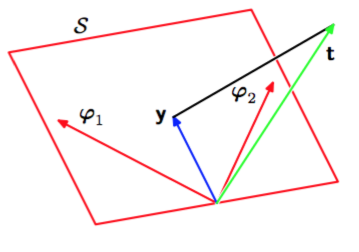
\includegraphics[width=5cm]{Figure2}
\caption{Examples of basis functions.}
%\label{Figure2}
\end{figure}

In an N-dimensional space whose axes are the value of $t_1,\cdots,t_N$. The least-squares regression function is obtained by finding the orthogonal projection of the data vector $\bm{t}$ onto the subspace spanned by the basis functions.

\end{frame}


\subsection{Sequential learning} 

%------------------------------------------------

\begin{frame}
\frametitle{Sequential Learning}
Batch techniques, such as the maximum likelihood solution which can process large dataset in one go, if the dataset if sufficiently large, it may be worthwhile to use sequential algorithms, known as \textit{on-line} algorithm. Sequential learning is also appropriate for real-time applications.\\~\\

\textit{Stochastic gradient descent} is applied. If the error function  comprises a sum over data points $E = \sum_n E_n$, the update rule:

\begin{equation}
\bm{w}^{\tau+1}=\bm{w}^{\tau}-\eta \nabla E_n
\end{equation}\\~\\

For the case of  the sum-of-squares error function, this gives:
\begin{equation}
\bm{w}^{\tau+1}=\bm{w}^{\tau}-\eta (t_n - \bm{w}^{(\tau)T}\phi_n)\phi_n
\end{equation}

\end{frame}


%------------------------------------------------

\begin{frame}
\frametitle{Regularized Least Squares I}
The regularization terms are added to the error functions. One of the simplest forms of regularizer is given by the sum-of-squares of the weight vector elements:
\begin{equation}
E_W(\bm{w} = \frac{1}{2}\bm{w}^T\bm{w})
\end{equation}

Consider the sum-of-squares error function with regularizer (quadratic regularizer):
\begin{equation}
 E = \frac{1}{2}\sum_{n=1}^{N}\{t_n-\bm{w}^T\bm{\phi}(\bm{x}_n)\}^2+\frac{\lambda}{2}\bm{w}^T\bm{w}
\end{equation}
 This choice of regularizer is known as \textit{weight decay}, because in sequential learning algorithms, it encourages weight values to decay towards zero.\\~\\
 
 Solving fro $w$ as the gradient of (12) equal to zero, we obtain:
 \begin{equation}
 \bm{w} = (\lambda \bm{I} + \bm{\Phi}^T \bm{\Phi})^{-1} \bm{\Phi}^T\bm{t}
 \end{equation}
 This represents a simple extension of the least-squares solution (8).
 
\end{frame}



\begin{frame}
\frametitle{Regularized Least Squares II}

\begin{figure}
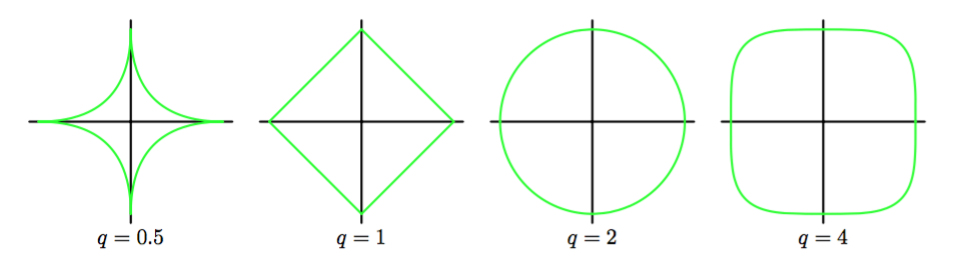
\includegraphics[width=12cm]{Figure3}
\caption{Contours of the regularization term for various values of the parameter q.}
%\label{Figure3}
\end{figure}

A more general regularizer is 
\begin{equation}
\frac{\lambda}{2} \sum_{j=1}^M|w_j|^q
\end{equation}
when q=2 corresponds to the quadratic regularizer in (12).\\~\\
\end{frame}
%------------------------------------------------

\begin{frame}
\frametitle{Regularized Least Squares III}


\begin{figure}
\begin{columns}
\column{.6\linewidth}
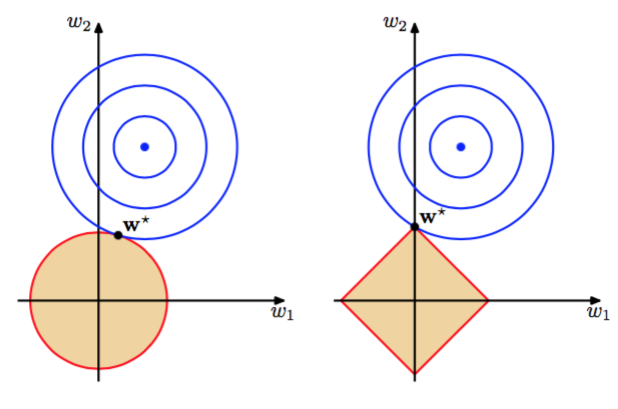
\includegraphics[width=7cm]{Figure4}
\column{.3\linewidth}
\caption{The  error function without regularization and the constraint region for quadratic regularizer (left) and lasso regularizer (right). We can see the $w$ in lasso equals to 0 make a sparse solution.}
%\label{Figure4}
\end{columns}
\end{figure}


The case of q=1 is known as the \textit{lasso} which leading to a \textit{sparse} model in which the corresponding basis functions play no role.
Regularization allows complex models to be trained on data sets of limited size without severe over-fitting, essentially by limiting the effective model complexity. However, the problem of determining the optimal model complexity is then shifted from one of finding the regularization coefficient $\lambda$.
\end{frame}


\begin{frame}
\frametitle{Multiple Outputs}
If the target value $t$ turns to a vector $\bm{t}$ which means multiple outputs. This could be done via multiple, independent regression problems.\\~\\

However, usually we use the same set of basis functions to model all components of the target value vector. Suppose we take the conditional distribution of the target vector to be an isotropic Gaussian of the form
\begin{equation}
p(\bm{t}|\bm{x},\bm{W},\beta)=\mathcal{N}(\bm{t}|\bm{W}\bm{\phi}(\bm{x}),\beta^{-1}\bm{I})
\end{equation}

The log likelihood function is then given by:
\begin{equation}
ln p(\bm{T}|\bm{X},\bm{W},\beta) = \sum_{n=1}^{N}\mathcal{N}(\bm{t}_n|\bm{W}^T \bm{\phi}(\bm{x}_n),\beta^{-1}\bm{I})
\end{equation}

and maximize this function with respect to $\bm{W}$.

\end{frame}



%------------------------------------------------
\section{Bias-Variance Decomposition} % Sections can be created in order to organize your presentation into discrete blocks, all sections and subsections are automatically printed in the table of contents as an overview of the talk
%------------------------------------------------

\begin{frame}
\frametitle{Bias-Variance trade-off}
The phenomenon of overfitting is an unfortunate property of maximum likelihood. Consider the Bayesian view of model complexity in depth. We consider a frequentist viewpoint of the model complexity issue, known as the bias-variance trade-off. \\~\\


Various loss functions leads to different  corresponding optimal prediction, once we are given the conditional distribution $p(t|x)$. A popular choice is  the square loss function, for which the optimal prediction is given by the conditional expectation -- we denote by $h(x)$ and is given by:
\begin{equation}
h(\bm{x})=\mathbb{E}(t|\bm{x})=\int tp(t|\bm{x})dt
\end{equation}

\end{frame}


\begin{frame}
\frametitle{Loss Function for Regression - Chap 1.5.5}
The decision stage consists of choosing a $y(\bm{x})$ of the value of $t$ for each input $\bm{x}$. Suppose we incur a loss $L(t,y(\bm{x}))$, the average or expected loss is given by:
\begin{equation}
\mathbb{E}[L]=\int \int L(t,y(\bm{x}))p(\bm{x},t)d\bm{x}dt
\end{equation}

Our goal is to choose $y(\bm{x})$ so as to minimize $\mathbb{E}[L]$, assume a flexible function $y(\bm{x})$, do this using the calculus of variations to give:

\begin{equation}
\frac{\partial \mathbb{E}[L]}{\partial y(\bm{x})} = 2 \int \{y(\bm{x})-t\}p(\bm{x},t)=0
\end{equation}

Solving for $y(\bm{x})$ and using the sum and product rules of probability, we obtain:
\begin{equation}
y(\bm{x})=\frac{\int tp(\bm{x},t)dt}{p(\bm{x})}=\int tp(t|\bm{x})dt=\mathbb{E}_t[t|\bm{x}]
\end{equation}
which is the conditional average of t conditioned on x and is known as the regression function.
\end{frame}



\begin{frame}
\frametitle{Loss Function for Regression - Chap 1.5.5}
\begin{figure}
\begin{columns}
\column{.6\linewidth}
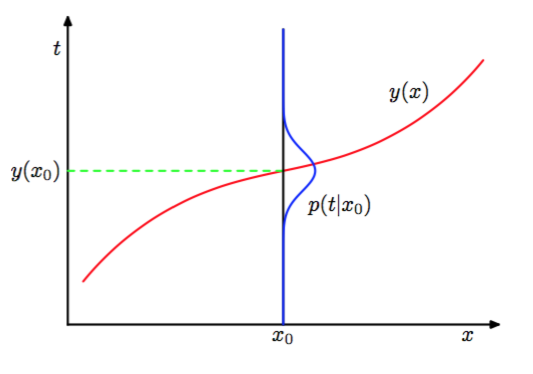
\includegraphics[width=7cm]{Figure5}
\column{.3\linewidth}
\caption{The regression function $y(x)$, which minimizes the expected squared loss, is given by the mean of the conditional distribution $p(t|x)$}
%\label{Figure5}
\end{columns}
\end{figure}

- It is easy to be extented into multiple target variables represented by the vector $\bm{t}$, in which case the optimal solution is the conditional average $y(\bm{x})=\mathbb{E}[\bm{t}|\bm{x}]$.

\end{frame}



\begin{frame}
\frametitle{Loss Function for Regression - Chap 1.5.5}
We can expand the square term as :

\begin{equation}
\{y(\bm{x})-t\}^2=\{y(\bm{x}-\mathbb{E}[t|\bm{x}]+\mathbb{E}[t|\bm{x}])-t\}^2
\end{equation}\\~\\

We use $\mathbb{E}[t|\bm{x}]$ to denote $\mathbb{E}_t[t|\bm{x}]$, and then performing the integral over t, the cross-term in (21) will vanish and then we have:

\begin{equation}
E[L]=\int \{y(\bm{x})-t\}^2p(\bm{x})d\bm{x}+\int var[t|\bm{x}]p(\bm{x})d\bm{x}
\end{equation}\\~\\

The function we seek to determine enters only in the first term, whch will be minimized when $y(\bm{x})$ is equal to $\mathbb{E}[t|\bm{x}]$, in which case this term will vanish. This is simply the result that we derived previously and that show that the optimal least squares predictor is given by the conditional mean. The second term is the variance of the distribution of t, averaged over $\bm{x}$.
\end{frame}




\begin{frame}
\frametitle{Expected squared loss}
So we can write the expected squared loss:
\begin{equation}
E[L]=\int \{y(\bm{x})-h(\bm{x})\}^2p(\bm{x})d\bm{x}+\int \int \{h(\bm{x}-t)^2\}p(\bm{x})d\bm{x}
\end{equation}\\~\\

The second term is independent of $y(\bm{x})$, arises from the intrinsic noise on the data and reprents the minimum achievable value of the expected loss.

For the first term, the smallest value is zero. If we had an unlimited supply of data, we might find the regression function $h(\bm{x})$ to any desired degree of accuracy, which represents the optimal choice for $y(\bm{x})$.\\~\\

However, in practice we have limited dataset of $\mathcal{D}$ containing $N$ data points, and consequently we do not know the regression function $h(\bm{x})$ exactly.
\end{frame}


\begin{frame}
\frametitle{Algorithm Assessment}
If we want to model the $h(\bm{x})$ using a parametric function $y(\bm{x},\bm{w})$ governed by vector $\bm{w}$, then from a Bayesian perspective the uncertainty in our model is expressed through a posterior distribution over $\bm{w}$.\\~\\

From the frequentist treatment, involves making a point estimate of $\bm{w}$ based on the data set $\mathcal{D}$, and tries instead to interpret the uncertainty of this estimate through the thought experiment:
\begin{enumerate}
\item suppose we had a large data sets with size N, and each draw independently from $p(t,\bm{x})$.
\item for the given dataset $\mathcal{D}$, we use learning algorithm obtain a prediction function $y(\bm{x};\mathcal{D})$.
\item different dataset, we have different prediction function.
\item then we have different values of squared loss.
\item the particular algorithm is then assessed by the average over the ensemble of datasets.
\end{enumerate}
\end{frame}



\begin{frame}
\frametitle{Bias-Variance in Expectation }
 Consider the integrand of the first term of $\mathbb{E}[L]$, for a particular data set $\mathcal{D}$ takes the form
 \begin{equation}
 \{y(\bm{x};\mathcal{D}-h(\bm{x}))\}^2
 \end{equation}
 we take its average over the ensemble of data sets. Because this quantity will be dependent on the particular data set $\mathcal{D}$.\\~\\
 
 We now take the expectation of this expression with respect to $\mathcal{D}$ and note that the final term will vanish , giving:
 \begin{equation}
 \begin{split}
 \mathbb{E}_{\mathbb{D}}[\{y(\bm{x};\mathcal{D})-h(\bm{x})\}]
 =\underbrace{\{\mathbb{E}_{\mathcal{D}}[y(\bm{x};\mathcal{D})]-h(\bm{x})\}^2}_{(bias)^2}+ \\\underbrace{\mathbb{E}_{\mathcal{D}}[\{y(\bm{x};\mathcal{D})-\mathbb{E}_{\mathcal{D}}[y(\bm{x};\mathcal{D})]\}^2]}_{variance}
 \end{split}
 \end{equation}
 
 We see that the expected squared difference between $y(\bm{x},\mathcal{D})$ and the regression function $h(\bm{x})$ can be expressed as the sum of two terms.
\end{frame}


\begin{frame}
\frametitle{Bias-Variance in Expectation }

 \begin{columns}[T]
\begin{column}{.47\textwidth}
\begin{block}{Various data points.}
% Your image included here
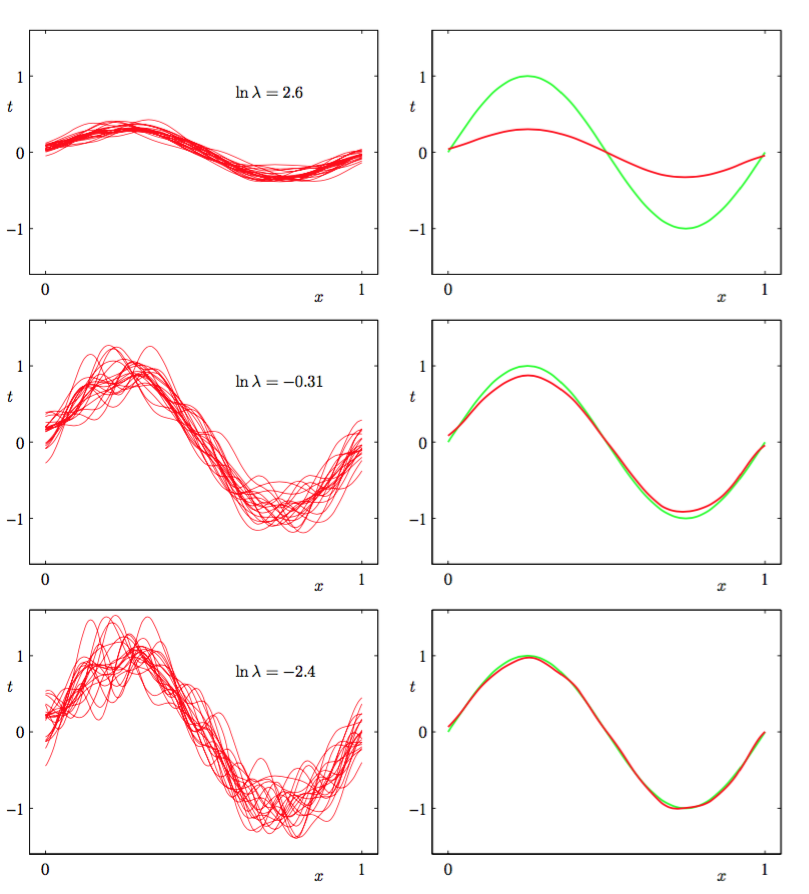
\includegraphics[width=\textwidth]{Figure6}

\end{block}
\end{column}


\begin{column}{.47\textwidth}
\begin{block}{Comparisons}
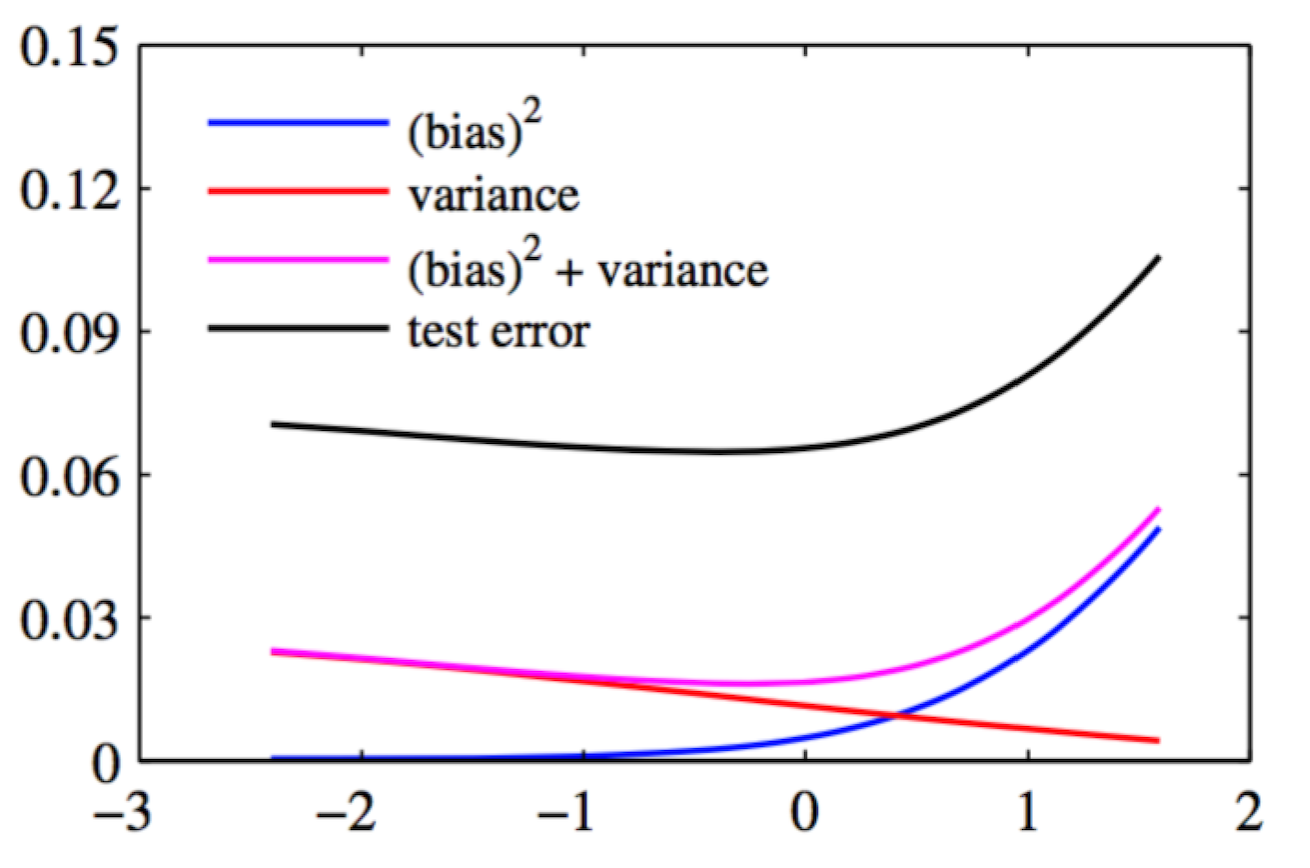
\includegraphics[width=\textwidth]{Figure7}

Illustration of the dependence of bias and variance on model complexity governed by a regularization parameter $\lambda$ and the results for $(bias)^2+variance$.

\end{block}
\end{column}
\end{columns}
\end{frame}


\begin{frame}
\frametitle{Bias-Variance in Expectation }
From the comparisons curve we can check the variations for different $\lambda$. When $\lambda$ is large (in the top row of last page left graph), we can see the red curves plot look similar in left column-- low variance,  but in the right column two curves are quite different -- high bias.\\~\\

In the bottom row which is quite different which $\lambda$ is small and we have large variance --  shown by the high variability between the red curves in the left plot, and low bias shown by the good fit to the regression function.\\~\\

Note that the result of averaging many solutions for the complex model with $M=25$ is a very good fit to the regression function.\\~\\

Indeed, a weighted averaging of multiple solutions lies at the heart of a Bayesian approach, with respect to the posterior distribution of parameters (not with respect to multiple data sets).
\end{frame}



%------------------------------------------------
\section{Bayesian Linear Regression} % Sections can be created in order to organize your presentation into discrete blocks, all sections and subsections are automatically printed in the table of contents as an overview of the talk
%------------------------------------------------


\subsection{Parameter distribution}

%------------------------------------------------
\begin{frame}
\frametitle{Parameter Distribution}


\end{frame}

\subsection{Predictive distribution}

%------------------------------------------------
\begin{frame}
\frametitle{Predictive Distribution}

\end{frame}
%------------------------------------------------


\subsection{Equivalent kernal}

%------------------------------------------------
\begin{frame}
\frametitle{Equivalent Kernal}

\end{frame}
%------------------------------------------------


\section{Bayesian Model Comparison}

%------------------------------------------------
\begin{frame}
\frametitle{Bayesian Model Comparison}

\end{frame}
%------------------------------------------------



\section{Evidence Approximation}

\subsection{Evaluation of Approximation Function}

%------------------------------------------------
\begin{frame}
\frametitle{Evaluation of Approximation Function}

\end{frame}
%------------------------------------------------

\subsection{Maximizeing the evidence function}

%------------------------------------------------
\begin{frame}
\frametitle{Maximizeing the Evidence Function}

\end{frame}
%------------------------------------------------


\begin{frame}
\frametitle{Bullet Points}
\begin{itemize}
\item Lorem ipsum dolor sit amet, consectetur adipiscing elit
\item Aliquam blandit faucibus nisi, sit amet dapibus enim tempus eu
\item Nulla commodo, erat quis gravida posuere, elit lacus lobortis est, quis porttitor odio mauris at libero
\item Nam cursus est eget velit posuere pellentesque
\item Vestibulum faucibus velit a augue condimentum quis convallis nulla gravida
\end{itemize}
\end{frame}

%------------------------------------------------

\begin{frame}
\frametitle{Blocks of Highlighted Text}
\begin{block}{Block 1}
Lorem ipsum dolor sit amet, consectetur adipiscing elit. Integer lectus nisl, ultricies in feugiat rutrum, porttitor sit amet augue. Aliquam ut tortor mauris. Sed volutpat ante purus, quis accumsan dolor.
\end{block}

\begin{block}{Block 2}
Pellentesque sed tellus purus. Class aptent taciti sociosqu ad litora torquent per conubia nostra, per inceptos himenaeos. Vestibulum quis magna at risus dictum tempor eu vitae velit.
\end{block}

\begin{block}{Block 3}
Suspendisse tincidunt sagittis gravida. Curabitur condimentum, enim sed venenatis rutrum, ipsum neque consectetur orci, sed blandit justo nisi ac lacus.
\end{block}
\end{frame}

%------------------------------------------------

\begin{frame}
\frametitle{Multiple Columns}
\begin{columns}[c] % The "c" option specifies centered vertical alignment while the "t" option is used for top vertical alignment

\column{.45\textwidth} % Left column and width
\textbf{Heading}
\begin{enumerate}
\item Statement
\item Explanation
\item Example
\end{enumerate}

\column{.5\textwidth} % Right column and width
Lorem ipsum dolor sit amet, consectetur adipiscing elit. Integer lectus nisl, ultricies in feugiat rutrum, porttitor sit amet augue. Aliquam ut tortor mauris. Sed volutpat ante purus, quis accumsan dolor.

\end{columns}
\end{frame}


\begin{frame}
\frametitle{Table}
\begin{table}
\begin{tabular}{l l l}
\toprule
\textbf{Treatments} & \textbf{Response 1} & \textbf{Response 2}\\
\midrule
Treatment 1 & 0.0003262 & 0.562 \\
Treatment 2 & 0.0015681 & 0.910 \\
Treatment 3 & 0.0009271 & 0.296 \\
\bottomrule
\end{tabular}
\caption{Table caption}
\end{table}
\end{frame}

%------------------------------------------------

\begin{frame}
\frametitle{Theorem}
\begin{theorem}[Mass--energy equivalence]
$E = mc^2$
\end{theorem}
\end{frame}

%------------------------------------------------

\begin{frame}[fragile] % Need to use the fragile option when verbatim is used in the slide
\frametitle{Verbatim}
\begin{example}[Theorem Slide Code]
\begin{verbatim}
\begin{frame}
\frametitle{Theorem}
\begin{theorem}[Mass--energy equivalence]
$E = mc^2$
\end{theorem}
\end{frame}\end{verbatim}
\end{example}
\end{frame}

%------------------------------------------------

\begin{frame}
\frametitle{Figure}
Uncomment the code on this slide to include your own image from the same directory as the template .TeX file.
%\begin{figure}
%\includegraphics[width=0.8\linewidth]{test}
%\end{figure}
\end{frame}

%------------------------------------------------

\begin{frame}[fragile] % Need to use the fragile option when verbatim is used in the slide
\frametitle{Citation}
An example of the \verb|\cite| command to cite within the presentation:\\~

This statement requires citation \cite{p1}.
\end{frame}

%------------------------------------------------

\begin{frame}
\frametitle{References}
\footnotesize{
\begin{thebibliography}{99} % Beamer does not support BibTeX so references must be inserted manually as below
\bibitem[Smith, 2012]{p1} John Smith (2012)
\newblock Title of the publication
\newblock \emph{Journal Name} 12(3), 45 -- 678.
\end{thebibliography}
}
\end{frame}

%------------------------------------------------

\begin{frame}
\Huge{\centerline{The End}}
\end{frame}

%----------------------------------------------------------------------------------------

\end{document} 